\chapter{設計及模擬環境}
%\renewcommand{\baselinestretch}{10.0} %設定行距

%----------------設計環境---Solid Edge-----------------%
\section{設計環境---Solid Edge}
Solid Edge為一個由西門子PLM開發的三維特徵造型實體軟體,設計者可以通過輸入參數以生成3D模型或是分析模型等動作,在2017年,Solid Edge也引進創成式設計功能,能夠依照多次疊代運算產生最終的優化結果。\
用Solid Edge作為分析軟體有幾特點及因素,其一為分別有兩種建模方式,對於繪製模型或修改都有跟高的便利性,其二可以直接對繪製零件進行有限元分析及創成式設計,可以直接將模型透過3D打印出來,不必經過其他軟體。\
\subsection{Solid Edge特徵建模}
為兩種Solid Edge的建模方式,可以根據繪製情況選取,在不同的情況下可隨時過渡到同步建模或過渡到順序建模
\begin{enumerate}
\item 順序建模:根據歷程記錄,可以返回到特徵建立過程的任何步驟,以編輯順序特徵。
\item 同步建模:定義特徵形狀的面的集合,未保留同步特徵的建立方式歷程記錄。
\end{enumerate}
順序建模環境中,顯示順序和同步特徵。\
同步建模環境中,順序建模特徵顯示為透明。\

%---------------路徑模擬-----Geogebra------------------%
\section{路徑模擬-----Geogebra}
誕生於2002年奧地利薩爾茨堡,其名稱由Geometry(幾何)和Algebra(代數)的混合詞,為一款動態幾何代數軟體,其特點為建立幾何物件,並保持其中連結關係,可以快速進行模擬計算並製作簡單動畫,作為教學演示軟體。\

%---------------運動模擬-----CoppeliaSim------------------%
\section{運動模擬-----CoppeliaSim}
在此專題中,CoppeliaSim為我們提供了良好的模擬環境,透過帶入Solid Edge的模型,可以更加直觀的觀察到步行機構的運動軌跡,利用Python或是Lua程式,在開發環境趨近於現實的軟體中,有著相當大的自由度,透過崁入式腳本、插件、Remote API客戶端,能對零件進行控制,每個轉軸、連桿、控制器等都可以在裡面持續調整且設定,對尺寸及建模進行運動優化、調整提供了許多便利性,也節省多次修改實體模型的費用。\\

\subsection{常用功能則}
以下為CoppeliaSim簡單介紹

\begin{figure}[hbt!]
\center
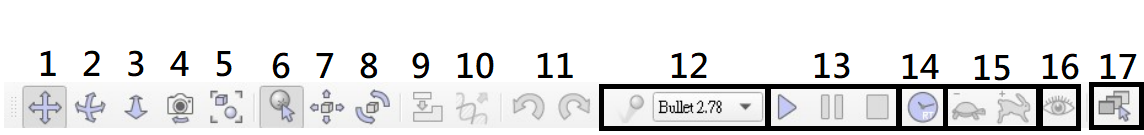
\includegraphics[width=13cm]{coppeliasim常用功能}
\caption{\Large CoppeliaSim常用功能}
\label{coppeliasim常用功能}
\end{figure}

\begin{table}[htbp]
  \centering
  \large
  \setlength{\tabcolsep}{0.75cm}
  \begin{tabular}{|c|c|c|c|}
    \hline
    代號 & 功能說明 & 代號 & 功能說明 \\
    \hline
    1 & 畫面平移 & 10 & 複製所有設定 \\
    \hline
    2 & 畫面旋轉 & 11 & 回復/取消回復 \\
    \hline
    3 & 畫面縮放 & 12 & 物理引擎選擇 \\
    \hline
    4 & 畫面視角 & 13 & 開始/暫停/停止 模擬 \\
    \hline
    5 & 畫面縮放至適當大小 & 14 & 即時模擬切換 \\
    \hline
    6 & 選取物件 & 15 & 模擬速度增減 \\
    \hline
    7 & 移動物件 & 16 & 視覺化 \\
    \hline
    8 & 旋轉物件 & 17 & 場景選擇 \\
    \hline
    9 & 加入/移出 樹狀結構 & & \\
    \hline
  \end{tabular}
\end{table}
\newpage

\begin{figure}[hbt!]
\center
\includegraphics[width=11cm]{CoppeliaSim}
\caption{\Large CoppeliaSim Logo}
\end{figure}
\subsection{RemoteAPI}
RemoteAPI(Remote Application Programming Interface) 為CoppeliaSim API 框架之一,開發者可以使用自己熟悉的語言來編寫遠程通信的代碼,此框架允許應用程式在不同環境中通信及交互,使開發者可以訪問遠程計算資源及服務,實現分部式系統及協同處理、集成應用等功能。\

\section{程式控制--Python}
Python為創始人Guido van Rossum(吉多·范羅蘇姆)在1989年決心開發的指令解釋碼模式已成為ABC語言的繼承者,並打算用其替代Unix shell和C語言來進行系統管理。\

為一開源並可擴充的語言,Python提供了豐富的API及工具,提供使用者能輕鬆使用的環境,其設計理念為<優雅><明確><簡單>\
在很多作業系統中,python被整合在其中為標準的系統元件,因此可在多個作業系統中運行,且能直接執行程式碼並即時查看成果,且在網路開發、數值分析、自動化測試等,其廣泛的應用領域和靈活性、不同環境中共享代碼,成為許多開發者及科學家的首選語言。\

\section{有限元素分析}
\begin{enumerate}
\item Solid Edge
關於有限元素分析,利用了Solid Edge作為我們的分析環境,選擇的原因在於模型是由Solid Edge建模的,繪製草圖完畢能夠直接對零件進行分析,不用在不同軟體中來回切換,透過新建的研究並定義材料或新增材質,設定負載位置,即可方便的對模型進行分析。\
Solid Edge也能對零件直接進行創成式設計,即為在有限元素法分析過後,軟體經過多層的代數運算,在模型上新增或除料,對比之前工程師需要經過長久計算出可適用的模型,創成式設計大幅減少設計及時間成本,得益於近幾年電腦快速的發展,複雜的運算及設計通通可以透過創成式設計生成,不再受限於設計師的想法或經驗,並可以快速產生多個模型提供挑選。\
\item Ansys
\end{enumerate}
ANSYS Inc.成立於1970年,主要是工程模擬軟體和技術的研發,目的為減少設計周期及降低設計成本,在有限元分析、流體力學計算、設計優化等領域都有發展,有豐富的工具及靈敏度和擴展性,被工程師及設計師廣泛的使用。\

\newpage
